\section*{Introduction}

DNA double-strand breaks (DSBs) pose a serious threat to the integrity of bacterial cells. They can arise from various sources such as gamma radiation, antibiotic exposure, or collision of the replication fork with DNA-bound proteins. In \emph{E. coli}, DSB repair is initiated by the RecBCD complex. However, different sources of DSBs can lead to different repair pathways, as illustrated on Figure \ref{Fig:DSB_scheme}.

In the case of a two-sided DSB (Figure \ref{Fig:DSB_scheme}A), created for example by radiation or antibiotics, the break is first recognised by the RecBCD complex, which will bind to it and start translocating along the DNA at a speed of $\sim$1.5 kb/s, thanks to its combined 5' and 3' helicase activities. While translocating, RecBCD will digest both DNA strands until it meets a specific 8-base pair sequence (5'-GCTGGTGG-3') called Chi-site. Upon recognition of the Chi-site, RecBCD will pause briefly before resuming translocation, albeit with modified nuclease activity: the 5' DNA end will be degraded more slowly, and the 3' end will not be degraded at all, leading to a 3' DNA overhang. Of note, Chi recognition by RecBCD is not systematic, and will only occur with a $\sim$XX\% probability. As RecBCD creates the 3' overhang, the nuclease domain of its RecB subunit will promote loading of the RecA protein onto the single-stranded DNA (ssDNA). The resulting RecA-DNA nucleoprotein filament will be used as a template to search for an intact homologous sequence and perform homologous recombination.

Another frequent cause of DSB formation in \emph{E. coli} is the collision of the replication fork with DNA-bound proteins (Figure \ref{Fig:DSB_scheme}B), which has been reported to occur in $\sim$18\% of cells per cell cycle.\cite{Sinha2018} When the replication fork collides with a DNA-bound protein, it can lead to the disassembly of the replisome. The resulting Y-shaped DNA structure is then bound by the RuvAB complex, which will pull the DNA strands (in a process called "branch migration") to create a "chicken-foot" four-way DNA structure. The free end of this structure (DNA tail) is bound by RecBCD, which will either (i) digest the whole DNA tail and displace RuvAB, allowing the replisome to be re-loaded, or (ii) recognise a Chi-site and load the RecA protein onto the 3' end of the DNA tail. Since this part of the DNA was recently replicated, a homologous sequence is necessarily present in close proximity, and can be used for homologous recombination.

In the case of fork collisions, the DSB repair process is expected to occur faster than in the case of a two-sided break caused by antibiotics or radiation. Since the DNA tail is only a few kilobases long, its full digestion by RecBCD would only take a few seconds, and if a Chi-site is recognised and RecA loaded, the close proximity of a homologous sequence should ensure rapid homology searching. In the case of a two-sided break however the homologous sequence is not guaranteed to be nearby, and the homology search can take several minutes.\cite{Wiktor2021}

\begin{figure*}[htbp]
    \centering
    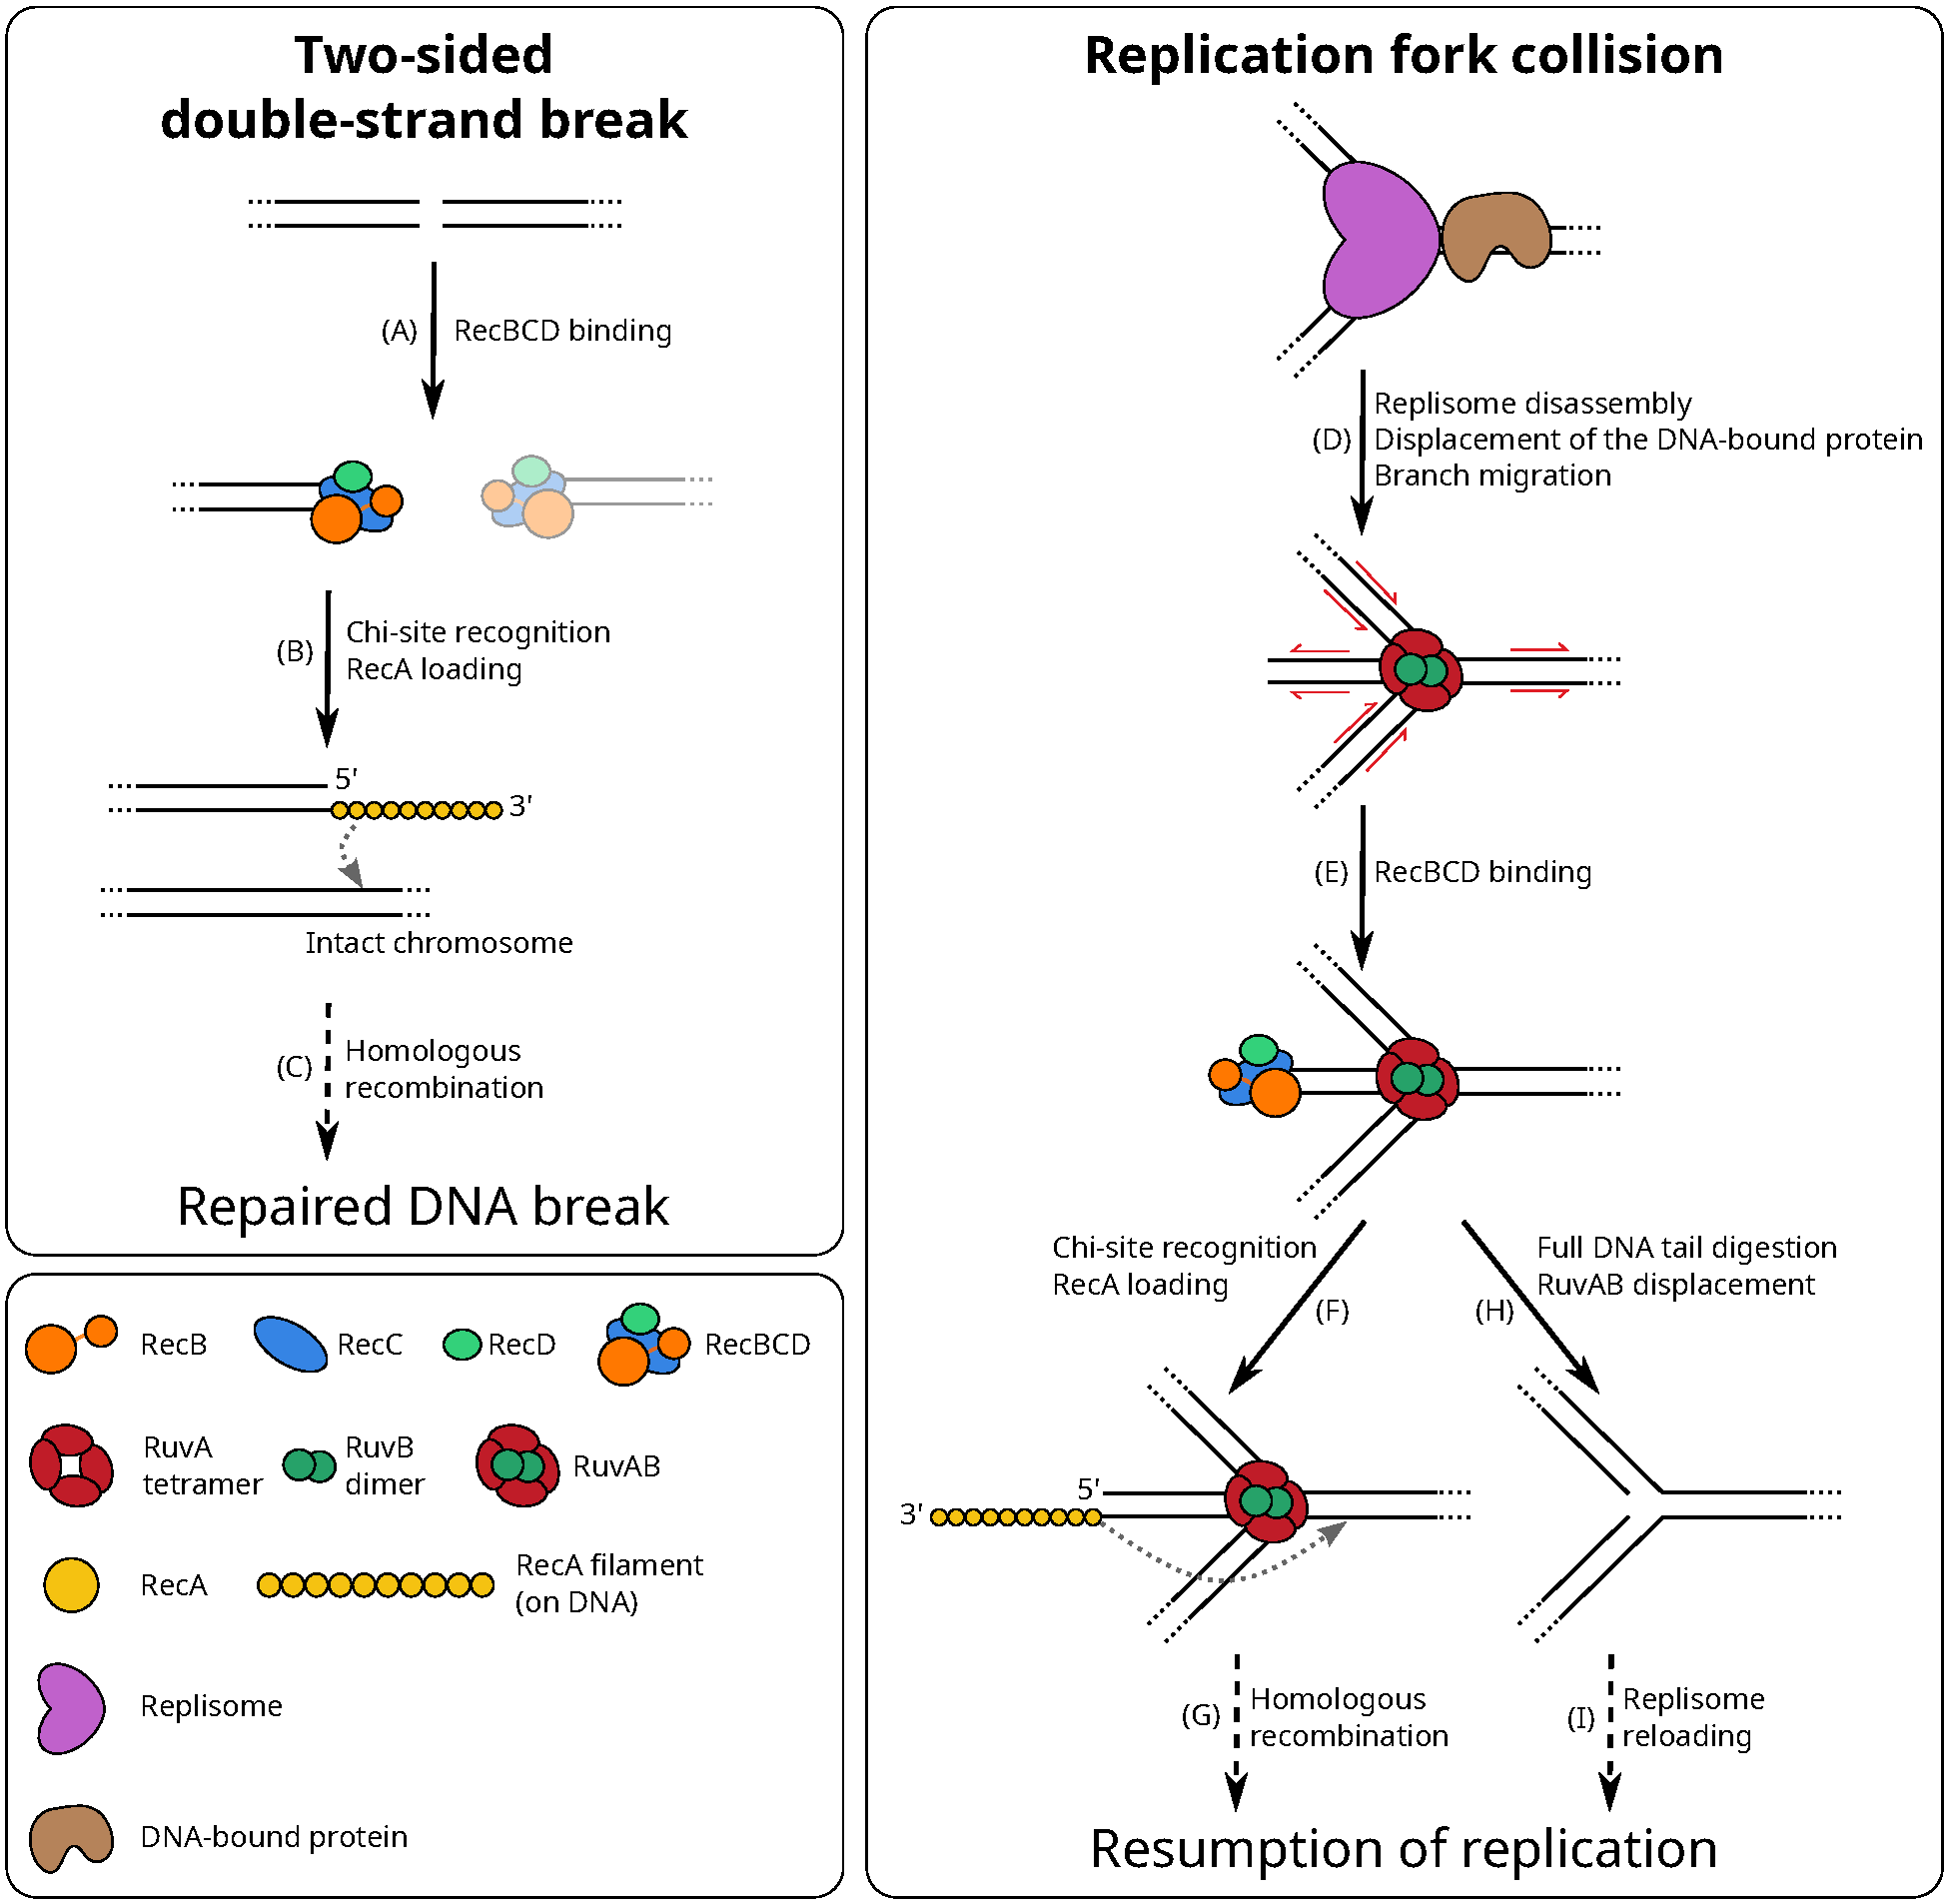
\includegraphics[width=.8\textwidth]{Figures/DSB_scheme.pdf}
    \caption{Double-strand break repair by RecBCD in \emph{E. coli}, in the case of a two-sided break (A), and in the case of replication fork collision (B).}
    \label{Fig:DSB_scheme}
\end{figure*}

% Add something about drecA and RecB1080 here (how are the pathways disturbed?)
Mutants in the repair pathway will deal differently with these types of damage. Cells that are \emph{recA}-deficient (\dreca) will be entirely unable to repair two-sided DSBs, and the prolonged action of RecBCD on the DNA will result in the digestion of large parts of the chromosome. \emph{recA}-deficient cells are however capable of repairing DSBs arising from fork reversal, thanks to RecBCD's exonuclease activity (Figure \ref{Fig:DSB_scheme}B, reaction G). The $D_{1080} \rightarrow A$ point mutation in the RecB subunit of the RecBCD complex (\teneighty) abolishes RecB's nuclease activity, as well as its ability to load the RecA protein on DNA. The other activities of the complex (DSB recognition, DNA unwinding, Chi-recognition) are unaffected. Despite the loss of its RecA loading activity, the \teneighty\ mutant is still able to repair two-sided DSBs. \teneighty CD will unwind DNA at the break without degrading it, and the Single-Strand Binding protein (SSB) will coat the 3' ssDNA, while the RecJ exonuclease degrades the 5' ssDNA. Finally, the RecFOR complex will displace SSB and load RecA, allowing for homologous recombination to occur. This process allows the \teneighty\ mutant to repair both two-sided DSBs and DSBs generated through replication fork collision, albeit at a slower rate. Of note, a \dreca-\teneighty double-mutant, which lacks both the RecA protein and RecB's nuclease activity, would be entirely unable to repair both types of DSBs.

% Antibiotics such as ciprofloxacin can cause massive amounts of damage
% Cipro poisons gyrase, which forms a covalent complex on DNA
% How this forms DSBs is unclear, could involve fork reversals and/or 2-sided DSBs created by the removal of the poisoned gyrase (with contribution of ExoVII)
% How does the cell deal with that damage?
Ciprofloxacin is an antibiotic of the fluor\-quinolones family, which causes DSBs. Im \emph{E. coli}, it does so by binding covalently to Topoisomerase II (CHECK), and trapping it in a DNA-bound conformation. Even though it is known that ciprofloxacin creates DSBs that are repaired by RecBCD, the exact mechanism through which the DSBs are created is still unclear. Since the poisoned gyrase is tightly bound to DNA, it might cause replication fork collisions, and the subsequent repair of a chicken foot structure (Figure \ref{Fig:DSB_scheme}B). The ciprofloxacin-poisoned gyrase is trapped in the "open" stage of its catalytic cycle, where it holds together two disjointed DNA ends. Therefore, upon removal of the gyrase (which likely involves the ExoVII nuclease), we can reasonably expect the formation of a two-sided DSB. It is likely that in fast-growing cells, which contain multiple replication forks, both processes are taking place.

% We use different antibiotic concentrations to see the difference between low and high amounts of damage
% We look at our metrics over time to see how the damage is dealt with
% We use mutants to assess the importance of different parts of the repair mechanism


% Details about the microscopy technique we use (enhanced localisation microscopy)


% In this paper, we aim to give more insight into specific steps of DSB repair
% NOVELTY: in-vivo + cipro + time-lapse imaging
% RecBCD binding time
% What happens when damage is too extensive to be repaired


